

%-------------------------------------------------------------------------------
% Dokumenten Klasse
\documentclass[
	final,
	a4paper,
	oneside,
	parskip=full,
	headings=standardclasses,
	headings=big,
	pointednumbers
]{scrartcl}

%-------------------------------------------------------------------------------
% Packete nutzen
\usepackage[T1]{fontenc}
\usepackage[utf8]{inputenc}
\usepackage[left=20mm,right=25mm,top=20mm,bottom=25mm]{geometry}
\usepackage{amsmath}
\usepackage{amssymb}
\usepackage{mathtools}

%-------------------------------------------------------------------------------
% TikZ
\usepackage{tikz}
\usetikzlibrary{positioning, arrows, decorations, calc}


\begin{document}

    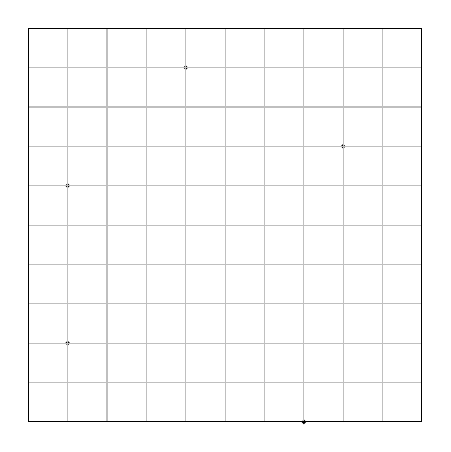
\begin{tikzpicture}[]
        \def\xlines{10}
        \def\ylines{10}
        \def\raster{5mm}

        \coordinate (A) at (7*\raster,0*\raster);
        \coordinate (B) at (8*\raster,7*\raster);
        \coordinate (C) at (4*\raster,9*\raster);
        \coordinate (D) at (1*\raster,6*\raster);
        \coordinate (E) at (1*\raster,2*\raster);

        \foreach \point in {A,B,C,D,E}{
            \draw[black, fill=black] (\point) circle (0.2mm);
        }

        % draw vertical lines
        \foreach \x in {0,...,\xlines}
        {
            \draw[lightgray] (\x * \raster, 0mm) -- (\x * \raster, \ylines * \raster);
        }

        % draw horizontal lines
        \foreach \y in {0,...,\ylines}
        {
            \draw[lightgray] (0mm, \y * \raster) -- (\xlines * \raster, \y * \raster);
        }

        % border
        \draw[black] (0mm, 0mm) -- (\xlines * \raster, 0mm);
        \draw[black] (0mm, 0mm) -- (0mm, \ylines * \raster);
        \draw[black] (\xlines * \raster, 0mm) -- (\xlines * \raster, \ylines * \raster);
        \draw[black] (0mm, \ylines * \raster) -- (\xlines * \raster, \ylines * \raster);
    \end{tikzpicture}

    \iffalse
    \begin{tikzpicture}[]
        \def\xlines{10}
        \def\ylines{10}
        \def\raster{5mm}

        \coordinate (A) at (7,0);
        \coordinate (B) at (8,7);
        \coordinate (C) at (4,9);
        \coordinate (D) at (1,6);
        \coordinate (E) at (1,2);

        \foreach \point in {A,B,C,D,E}{
            \draw[black] 
                let \p1 = (\point)
                in
                (\x1*\raster, \y1*\raster) circle (1mm);
        }

        % draw vertical lines
        \foreach \x in {0,...,\xlines}
        {
            \draw[lightgray] (\x * \raster, 0mm) -- (\x * \raster, \ylines * \raster);
        }

        % draw horizontal lines
        \foreach \y in {0,...,\ylines}
        {
            \draw[lightgray] (0mm, \y * \raster) -- (\xlines * \raster, \y * \raster);
        }

        % border
        \draw[black] (0mm, 0mm) -- (\xlines * \raster, 0mm);
        \draw[black] (0mm, 0mm) -- (0mm, \ylines * \raster);
        \draw[black] (\xlines * \raster, 0mm) -- (\xlines * \raster, \ylines * \raster);
        \draw[black] (0mm, \ylines * \raster) -- (\xlines * \raster, \ylines * \raster);
    \end{tikzpicture}
    \fi 

    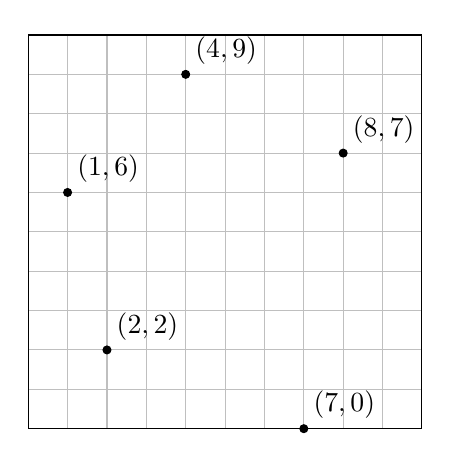
\begin{tikzpicture}[]
        \def\xlines{10}
        \def\ylines{10}
        \def\raster{5mm}

        \coordinate (A) at (7*\raster,0*\raster);
        \coordinate (B) at (8*\raster,7*\raster);
        \coordinate (C) at (4*\raster,9*\raster);
        \coordinate (D) at (1*\raster,6*\raster);
        \coordinate (E) at (2*\raster,2*\raster);

        % draw vertical lines
        \foreach \x in {0,...,\xlines}
        {
            \draw[lightgray] (\x * \raster, 0mm) -- (\x * \raster, \ylines * \raster);
        }

        % draw horizontal lines
        \foreach \y in {0,...,\ylines}
        {
            \draw[lightgray] (0mm, \y * \raster) -- (\xlines * \raster, \y * \raster);
        }
        
        \foreach \point/\a/\b in {A/7/0,B/8/7,C/4/9,D/1/6,E/2/2}{
            \draw[black,fill=black]
                let \p1 = (\point)
                in (\x1, \y1) circle (0.5mm);
            \path
                let \p1 = (\point)
                in
                    node[above right] at (\x1, \y1) {$\left( \a, \b \right) $};
        }
        

        % border
        \draw[black] (0mm, 0mm) -- (\xlines * \raster, 0mm);
        \draw[black] (0mm, 0mm) -- (0mm, \ylines * \raster);
        \draw[black] (\xlines * \raster, 0mm) -- (\xlines * \raster, \ylines * \raster);
        \draw[black] (0mm, \ylines * \raster) -- (\xlines * \raster, \ylines * \raster);
    \end{tikzpicture}

    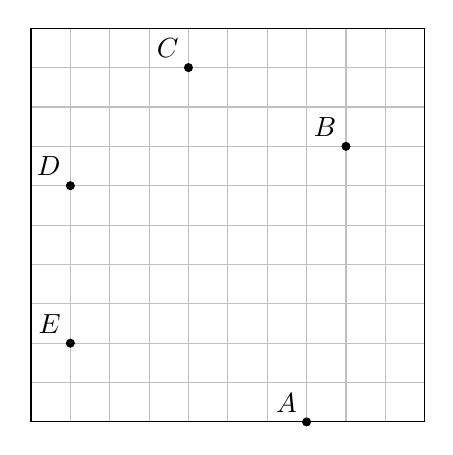
\begin{tikzpicture}[]
        \def\xlines{10}
        \def\ylines{10}
        \def\raster{5mm}

        \coordinate (A) at (7*\raster,0*\raster);
        \coordinate (B) at (8*\raster,7*\raster);
        \coordinate (C) at (4*\raster,9*\raster);
        \coordinate (D) at (1*\raster,6*\raster);
        \coordinate (E) at (1*\raster,2*\raster);

        % draw vertical lines
        \foreach \x in {0,...,\xlines}
        {
            \draw[lightgray] (\x * \raster, 0mm) -- (\x * \raster, \ylines * \raster);
        }

        % draw horizontal lines
        \foreach \y in {0,...,\ylines}
        {
            \draw[lightgray] (0mm, \y * \raster) -- (\xlines * \raster, \y * \raster);
        }

        
        \foreach \point/\num in {A/1,B/2,C/3,D/4,E/5}{
            \draw[black,fill=black] (\point) circle (0.5mm);
            \node[above left] at (\point) {$\point$};
        }
        

        % border
        \draw[black] (0mm, 0mm) -- (\xlines * \raster, 0mm);
        \draw[black] (0mm, 0mm) -- (0mm, \ylines * \raster);
        \draw[black] (\xlines * \raster, 0mm) -- (\xlines * \raster, \ylines * \raster);
        \draw[black] (0mm, \ylines * \raster) -- (\xlines * \raster, \ylines * \raster);
    \end{tikzpicture}


\end{document}